\documentclass[usenatbib]{mnras}
\usepackage[T1]{fontenc}
\usepackage{ae,aecompl}

\usepackage{graphicx}	% Including figure files
\usepackage{amsmath}	% Advanced maths commands
\usepackage{amssymb}	% Extra maths symbols
\usepackage{array}

\usepackage{multirow}
\usepackage{multicol}
\usepackage{blindtext}
\newcolumntype{?}{!{\vrule width 1pt}}
\newcommand{\Msun}{\,{\rm M}$_{\odot}$\,}
\newcommand{\Mpch}{\,{\rm Mpc}\,\ifmmode h^{-1}\else $h^{-1}$\fi}
\newcommand{\kpch}{\,{\rm kpc}\,\ifmmode h^{-1}\else $h^{-1}$\fi}
\newcommand{\kpc}{\,{\rm kpc}\,}
\newcommand{\kms}{\,{\rm km}\ s$^{-1}$\,}

%%%%%%%%%%%%%%%%%%% TITLE PAGE %%%%%%%%%%%%%%%%%%%
\title[Laniakea in a cosmological context]{The Laniakea supercluster in a cosmological context}
\author[Pe\~naranda-Rivera et al.]{
\parbox[t]{\textwidth}{
    {J. D. Pe\~naranda-Rivera $^1$,} 
    {D. L. Paipa-Le\'on$^{1}$,}
    {S. D. Hern\'andez-Charpak$^{1,2}$,}\\
    {J. E. Forero-Romero $^{1}$}
}
\\\\
$^{1}$ Departamento de F\'isica, Universidad de los Andes, Cra. 1
  No. 18A-10 Edificio Ip, CP 111711, Bogot\'a, Colombia \\
$^{2}$ Center for Neuroprosthetics and Brain Mind Institute, Swiss
  Federal Institute of Technology (EPFL), CH-1015, Lausanne,
  Switzerland\\  
}

% These dates will be filled out by the publisher
\date{Accepted XXX. Received YYY; in original form ZZZ}

% Enter the current year, for the copyright statements etc.
\pubyear{2019}


% Don't change these lines
\begin{document}
\label{firstpage}
\pagerange{\pageref{firstpage}--\pageref{lastpage}}
\maketitle

%%%%%====MYMARK========
\maketitle
\begin{abstract}
Galaxy superclusters can be defined as regions of converging galaxy
velocity flows. 
Such structures have quantifiable properties such as mass, volume and
shape. 
The most precise quantification of such an object has been done on our local supercluster, Laniakea. 
In this work the properties of Laniakea are compared to the
expectations from a Lambda Cold Dark Matter Universe. 
Cosmological N-body simulations are used in order to find cosmic flow
fields of dark matter halos and find the superclusters using a
watershed algorithm. 
In addition, the distributions of volume, mass and shape of the
superclusters found in those simulations are quantified and compared
with known values for Laniakea. 
In all those cases Laniakea is found in the tail of the distribution,
placing it as an atypical object in a cosmological context.  
\end{abstract}

\begin{keywords}
%%PREGUNTAR
%galaxies:supercluster --- simulation:cosmological --- filter:gaussian --- methods:numerical
\end{keywords}


%=========================================================================
%		PAPER CONTENT
%=========================================================================

%*************************************************************************

\section{Introduction}
% La introduccion y el abstract es lo ultimo que se escribe.

In 2014, astronomers used a map  of peculiar velocities of galaxies to
define the Laniakea supercluster of galaxies
\citep{2014Natur.513...71T}.  
Their main input was the Cosmicflows-2 catalog of distances and radial
velocities that provide them with coverage of distances up to 400\,Mpc. 
By applying a Wiener filter they obtained the reconstruction of the
3-dimensional velocity field. They defined and named our local galaxy supercluster, 
Laniakea, as the region within walls of divergence velocity.  
Laniakea thus represents the region of in-flowing peculiar velocities
that include the Milky Way. 

Laniakea has a very isotropic shape. 
Its radius is approximately $160$\,Mpc and encompasses a mass of
$\approx 10^{17}$\,\Msun.

We aim to quantify if Laniakea can be considered as a typical or atypical 
structure in our current cosmological conext.



\section{Numerical Setup}
\label{sec:numerical_setup}
\subsection{Cosmological N-body data}


In this paper we use simulations from the Abacus Cosmos project.
We use public data corresponding to dark matter only N-body
simulations executed on a cube of side length $720$\ \Mpch with
$1440^3$ particles.  
A set of these simulations assume a $\Lambda$CDM Planck 2015 cosmology
with different realizations for the initial conditions. 
Another set uses the same phases for the initial conditions, but
different cosmological parameters generated by a Latin hypercube
centered around the Planck 2015 parameters.  
The resolution of these simulations correspond to a DM particle mass
of $\sim 1 \times 10^{10}$ \Msun.
We use the public Friend-of-Friends catalogs at redshift $z=0.1$.
The halos included in those catalogs have a lower mass bound of 
maximum circular velocity of $V_{\rm circ}=50$\,\kms.
We trim these catalogs to halos with maximum circular velocity larger
than $300$ \kms. 
We have checked that changing changing this threshold to $200$ \kms does not
significantly impact our results. 



\subsection{Velocity interpolation, smoothing and divergence calculation}  

We interpolate the peculiar velocities for all halos on a grid using a
Cloud-In-Cell (CIC) scheme. 
We use a cubic grid with $360^3$ voxels, which means that each voxel
is a cube of $2$ \Mpch on a side.  
This resolution is deliberately smaller than the nominal resolution
used in the Wiener filter reconstruction performed on the
CosmicFlows-2 data used to define Laniakea. 
After the interpolation we smooth the velocity field using a gaussian
filter of physical scale $\sigma_s$.  
We compute the velocity divergence on this smooth velocity field. 
The purpose of this smoothing is to mimic the process of Wiener filter
reconstruction, which provides the equivalent of a smooth peculiar
velocity field. 
In explore different smoothing scales, $\sigma_s$/\Mpch, of $2$, $6$,
$10$, $14$ and $20$. 





\subsection{Watershed algorithm: Supercluster-Finder}

We use a watershed algorithm \citep{BeucherWatershed1979} on the velocity divergence field to find the
superclusters.
The algorithm segments the whole volume by assigning each voxel to a unique supercluster. 
Our implementation works as follows. 
We sweep the cells in the divergence grid from the lowest values to the highest, i.e. from
the high density regions with converging flows to the lowest density regions with divergent
flows.
For the $i$-th cell under consideration we check whether its 26 neighbors have already been assigned to a group. 
If all the neighbors are unassigned, then this $i$-th cell starts a
new group; if the majority of already assigned cells belongs to the
$n$-th group, then this cell belongs to that group.
In case of draw between groups, the cell is assigned to the supercluster with the lowest $n$ value.
At the end of the sweep all cells have been assigned to a group. 
In all our calculations we take periodical boundary conditions into
account.  
We highlight that once the divergence field is provided, this algorithm
does not have free parameters based either on divergence, density or distance thresholds. 
Finally, each group found by the algorithm is interpreted as a supercluster 
with a volume computed by counting the number of voxels belonging to it.

\section{Results}



\begin{figure}
    \centering
    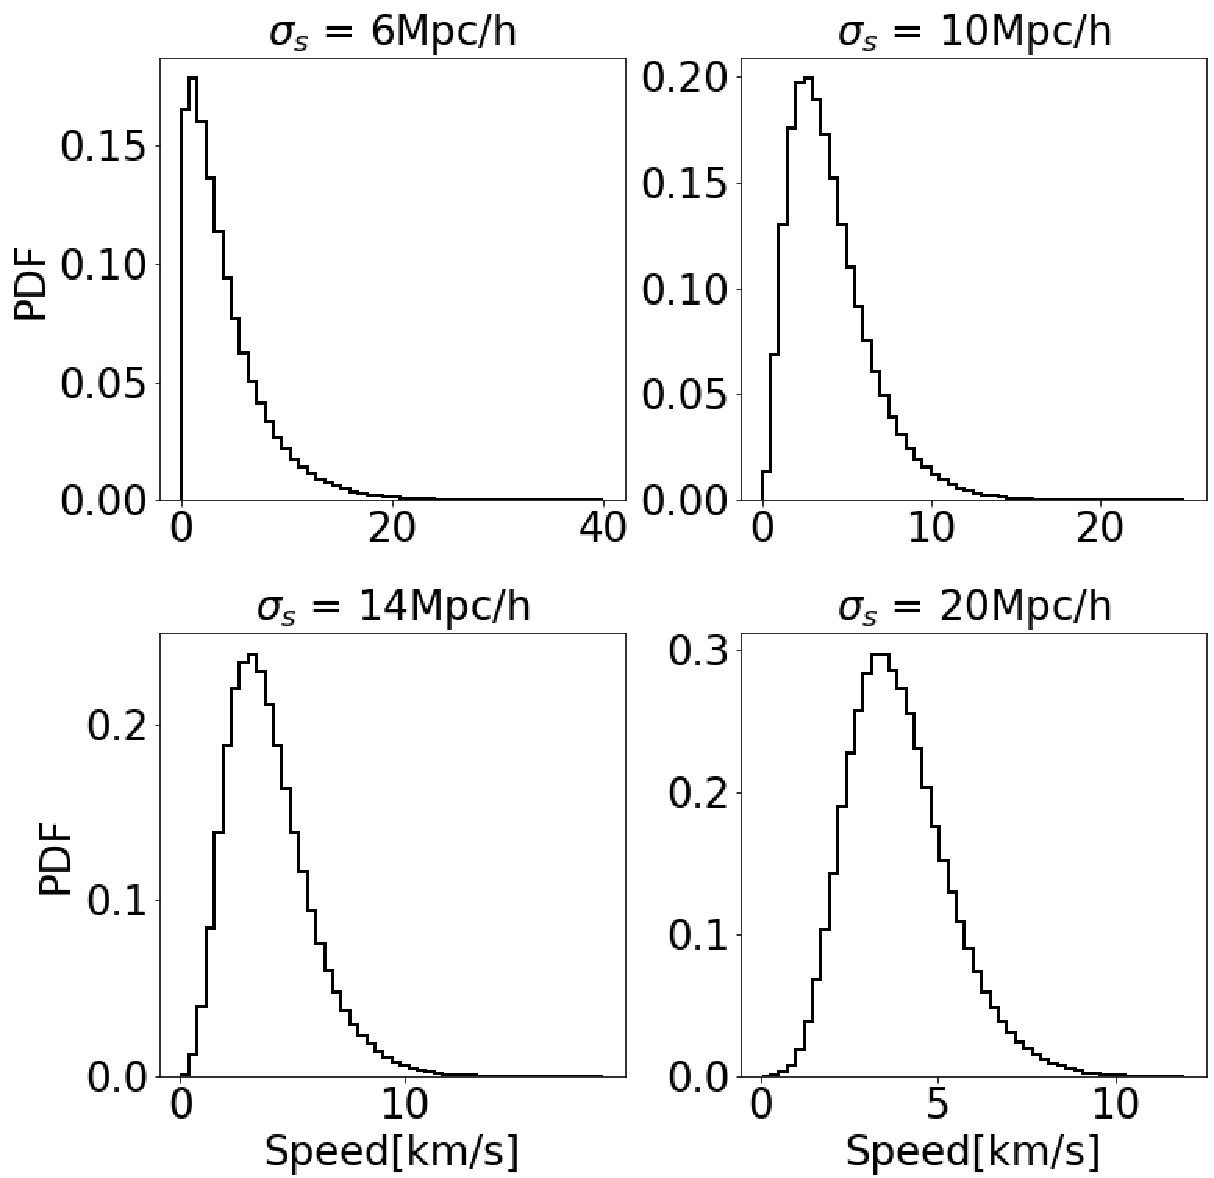
\includegraphics[width=240pt]{smooth_vel_dist.pdf}
    \caption{Distribution of the interpolated and smoothed velocity
      magnitude for different values of the smoothing scale $\sigma_{s}$.}
    \label{fig:smooth_vel_dist}
\end{figure}



\begin{figure}
    \centering
    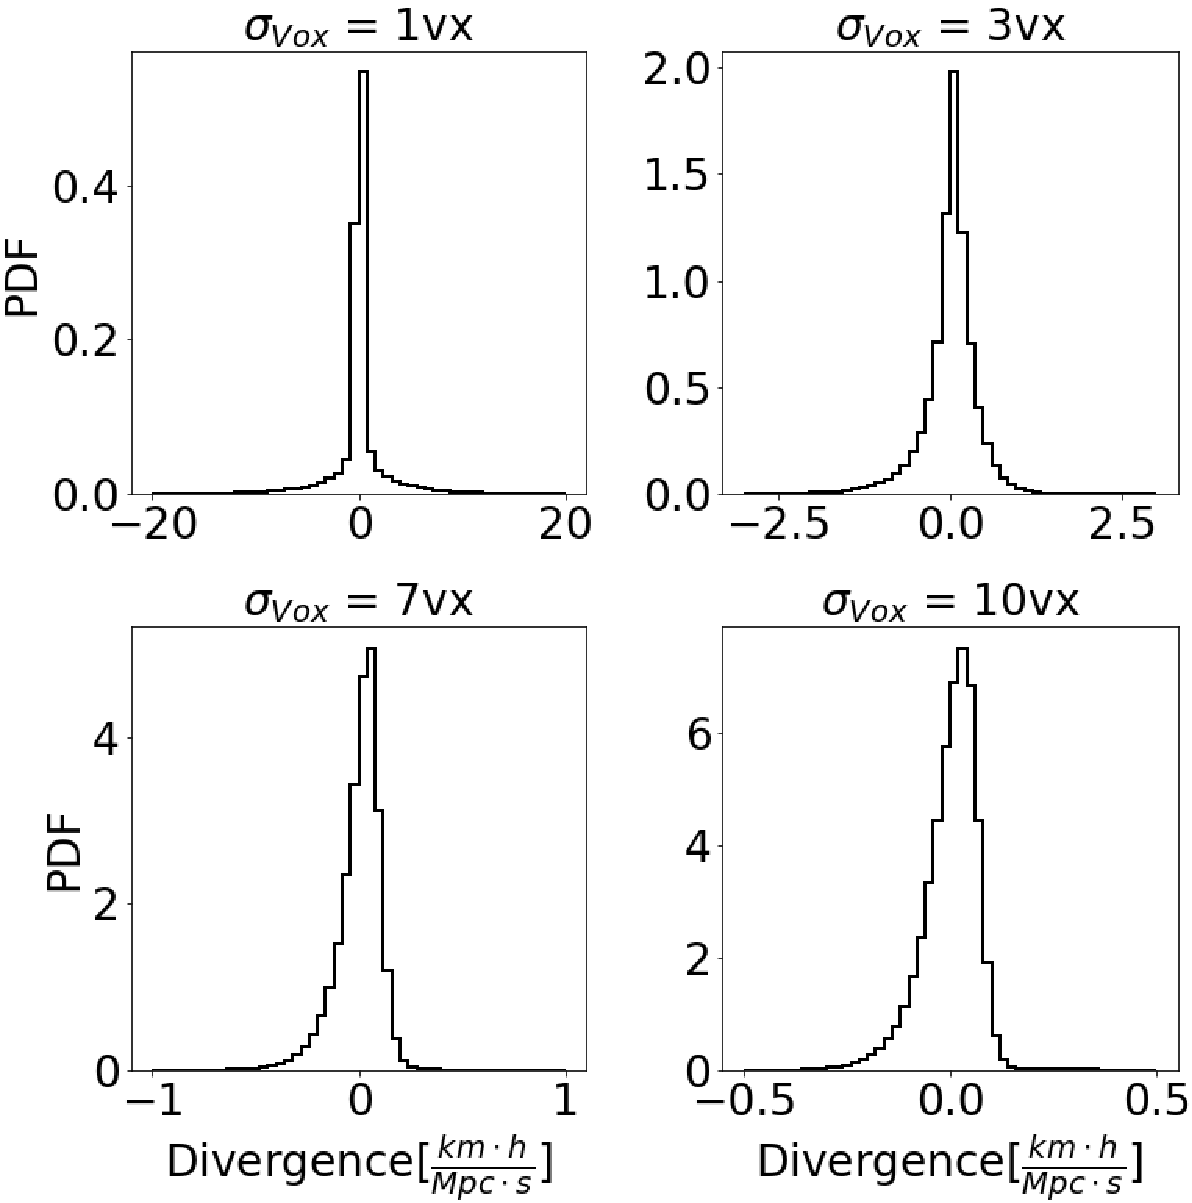
\includegraphics[width=240pt]{smooth_grad_dist.pdf}
    \caption{Distribution of the velocity divergence field
      for different values of the smoothing scale $\sigma_s$.}
    \label{fig:smooth_grad_dist}
\end{figure}



\begin{figure}
    \centering
    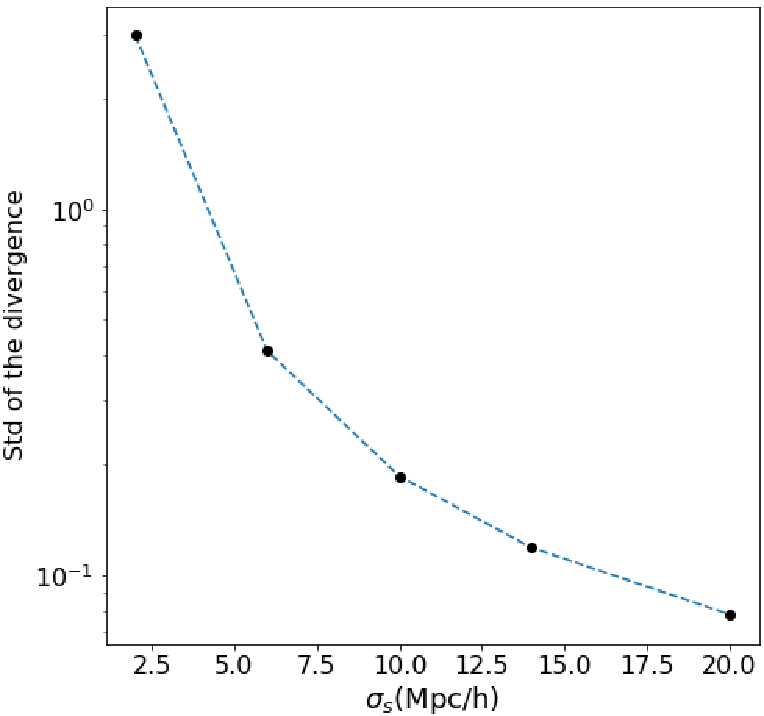
\includegraphics[width=240pt]{std_smooth.pdf}
    \caption{Standard deviation of the divergence field of
      as a function of the smoothing scale $\sigma_s$.}
    \label{fig:std_smooth}
\end{figure}



\begin{figure*}
    \centering
    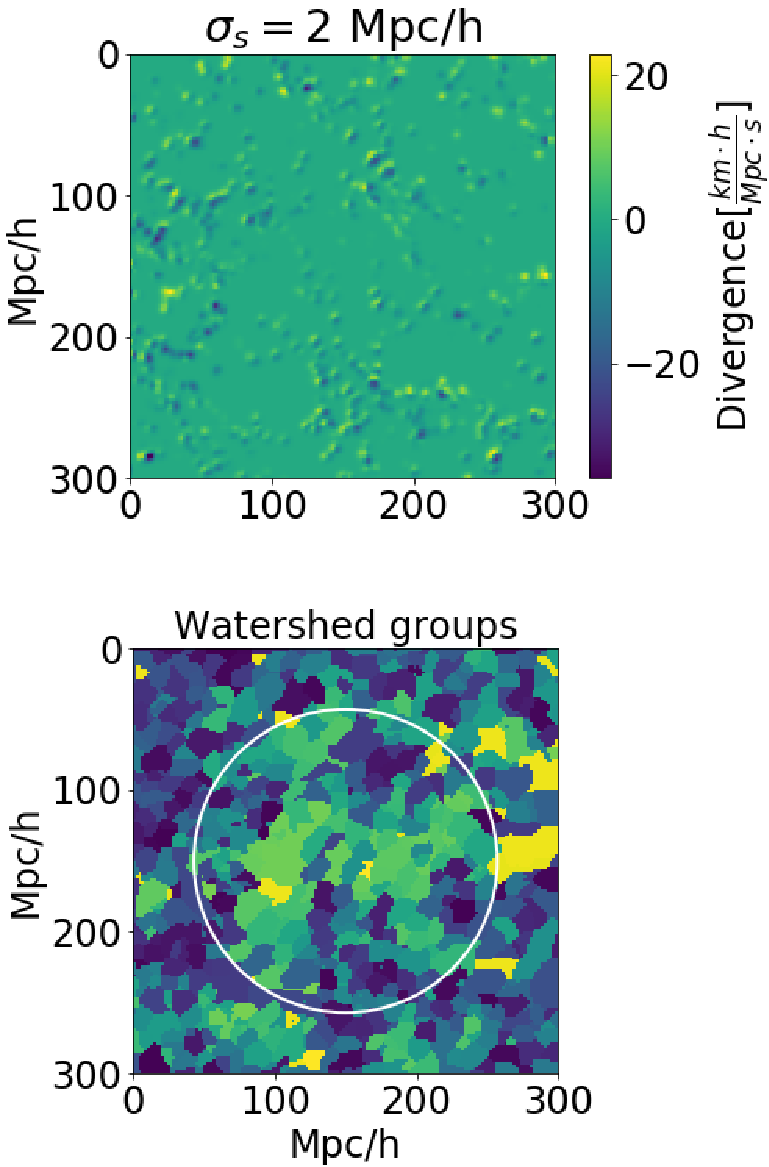
\includegraphics[width=220pt]{smooth_watershed_01.pdf}
    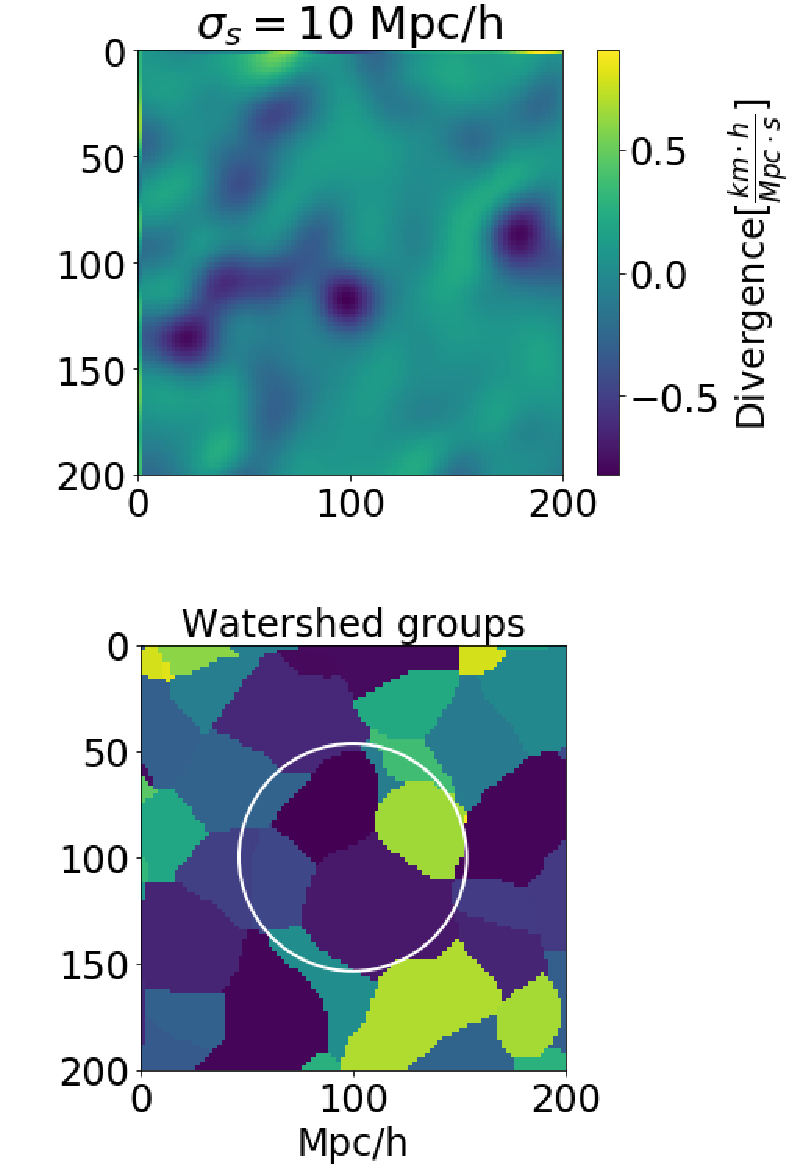
\includegraphics[width=211pt]{smooth_watershed_05.pdf}
    \caption{Figures on top show a random (300\,\Mpch)$^2$ cut on the
      X axis of the divergence grid for two different values of
      $\sigma_s$. Figures on the bottom show the classification made
      by the Watershed method for the two regions shown on top and
      where different superclusters have different colors. These two
      charts also contain a centered circle with the same diameter as
      Laniakea. It can be seen that Laniakea is much bigger than any
      other supercluster found using both $\sigma_s$.} 
    \label{fig:1Pert}
\end{figure*}



This section presents in the first place the influence of $\sigma_s$
on the velocity fields, its divergence and the resulting supercluster
segmentation. 
In a second stance we show the influence of cosmic variance and
different cosmological parameters on the volume distribution function
for superclusters. 

\subsection{Smoothing scale influence on the velocity and divergence fields}
\label{VDF effects}

Figure \ref{fig:smooth_vel_dist} shows the velocity norm distribution
for four different values of $\sigma_s$. 
As $\sigma_s$ increases the distribution becomes more symmetric with a
decreasing width, as expected.
The same trend is observed in Figure \ref{fig:smooth_grad_dist} for
the divergence of the velocity field.

This is neatly summarized in  Figure \ref{fig:std_smooth}.
The standard deviation of the divergence has a strong dependence on
the smoothing length.
The standard deviation goes from values of $3$  km s$^{-1}$ Mpc$^{-1}$ $h$ 
for a smoothing scale of $2$ \Mpch down to $0.075$ km s$^{-1}$
Mpc$^{-1}$ $h$ for a smoothing scale of $20$ \Mpch.
That means that increasing the smoothing scale by a factor of $8$
reduces the width of the divergence distribution by a factor of
$40$. 

\subsection{Smoothing scale influence on the resulting superclusters}
\label{sec:superclusters_influence}

The strong effects of the smoothing scale on the velocity and its
divergence is immediatly imprinted onto the results of the watershed
algorithm.


Finally, the influence of $\sigma_s$ on the sighting of structures
formation must be analyzed. This effects can be seen in Figure
\ref{fig:1Pert} where the same cross-section of the divergence field
grid is shown but smoothed with $\sigma_s$ = 2\,\Mpch and $\sigma_s$ =
10\,\Mpch (top diagrams). In addition, this chart presents the effects
of this parameter on the groups selected by watershed algorithm
(bottom diagrams), but this is discussed in the next section. These
plots show a random section of the divergence grid with size
(300\,\Mpch)$^2$. With small $\sigma_{s}$ many structures are visible
in a fine and defined network in the divergence grid, while large
$\sigma_{s}$ differentiates big structures of high accretion,
i.e. high negative, with barely any resolution of smaller
filaments. Also, using large $\sigma_{s}$ causes peak values of
divergence to be smoothed and values of the field move closer to  the
average value of the field.  








\subsubsection{Interpretation of low divergence regions}
Once the Gaussian process is realized in the simulations, several
regions of negative divergence are identified. These regions are
interpreted as places in space where matter is coming together at high
ratios. As a result, after the interpolation and smoothing are
executed, negative divergence regions are expected to have the largest
values of absolute velocities. These high negative divergence regions
can be observed in the divergence field chart using $\sigma_s =
10$\,\Mpch in figure \ref{fig:1Pert}. Notice how in these structures
the divergence is much more negative in the center of the
agglomerations than in the rest of the structure. The latter
corresponds to a structure formation process, interpreted in this
context as the region where a supercluster could possibly be, and will
be the first regions considered once we apply the watershed
algorithm. 


\subsection{$\sigma_s$ influence on the Watershed algorithm}


In the previous section we described how varying $\sigma_s$ has a
significant impact on the values of the velocity and divergence
fields. Since Watershed algorithm takes the divergence field and
segments it into disjoint groups (superclusters), it is expected that
$\sigma_s$ also modifies the result of the algorithm by
transitivity. In addition, we mentioned that increasing the Gaussian
length causes peak values of negative divergence to become large
structures with negative divergence. Therefore, since the algorithm
classifies according to the behaviour of these structures, if they get
bigger, superclusters detected by the algorithm will become greater
too. As a result, a drop on the number of superclusters detected must
be observed. The behaviour of the number of superclusters found as a
function of $\sigma_s$ is shown in figure \ref{fig:Nclusters}. Indeed,
we observe a considerable reduction of the number of superclusters
found when $\sigma_s$ is raised. In addition figures \ref{fig:1Pert}
and \ref{fig:HISTVMD2} shows the effects of changing the value of the
Gaussian length on the volumes of the superclusters detected. 

As mentioned in section \ref{VDF effects} figure \ref{fig:1Pert} shows
a random section of size (300\,\Mpch)$^2$ of the divergence grid using
$\sigma_s$ = 2\,\Mpch and $\sigma_s$ = 10\,\Mpch. Moreover, this
figure also presents the groups found by the algorithm corresponding
to this section, with a circle of the same diameter as Laniakea in the
middle of each chart. First, it can be seen that there is a clear
correspondence between the state of the divergence grid and the
structures found. If space is dominated by null divergence values and
small regions with negative divergence($\sigma_s = 2\,\Mpch$), small
groups will be detected. On the other hand, if the size of these
negative divergence regions is increased, large groups will be
detected by the algorithm. However, even when the value of $\sigma_s$
is raised from 2\,\Mpch to 10\,\Mpch, superclusters detected by
Watershed method are much smaller than the reported size of Laniakea
by \cite{2014Natur.513...71T}. The behaviour of the volume
distribution of the superclusters for different $\sigma_s$ values is
presented in figure \ref{fig:HISTVMD2}, where the same simulation is
smoothed using $\sigma_s$ = 2\,\Mpch, 6\,\Mpch, 14\,\Mpch and
20\,\Mpch. In addition, a vertical line is drawn to mark the reference
of the volume of Laniakea. For low $\sigma_s$ values, i.e. 2\,\Mpch
and 6\,\Mpch, no supercluster detected by the algorithm is as large as
Laniakea. In both cases Laniakea is found at the right side of the
distribution and is almost one or two orders of magnitude bigger than
the largest structures found for 2\,\Mpch and 6\,\Mpch
respectively. On the other hand, once we take values of $\sigma_s$
higher than 10\,\Mpch, Laniakea starts to be inside of the
distribution, as in $\sigma_s$ = 14\,\Mpch. Finally, we observe that
its volume becomes the must common one found by the algorithm when
$\sigma_s$ = 20\,\Mpch is taken. This result gives us a first hint of
the relation of Laniakea with the simulated superclusters found by
Watershed method. It seems to be that Laniakea is an atypical and very
large supercluster. We will delve into this topic in the following
section. 



\begin{figure}
    \centering
    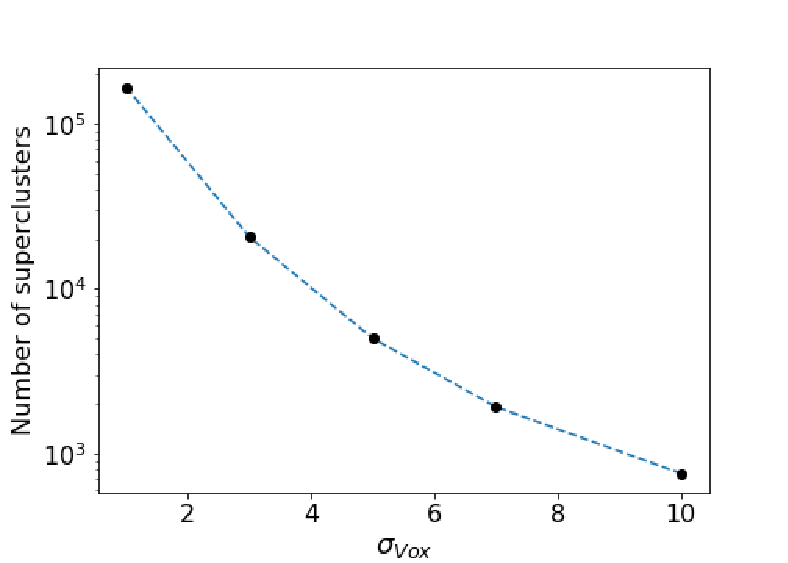
\includegraphics[width=240pt]{num_superclusters.pdf}
    \caption{Behaviour of the number of superclusters found in a
      simulation as a function of the smoothing scale parameter
      $\sigma_{Vox}$. Effectively a smaller $\sigma_{Vox}$ implies
      recognizing many more structures. 
This behavior was expected since each structure carries a smaller
volume and a larger number of them is required to fill the entire
space of the simulation.}  
    \label{fig:Nclusters}
\end{figure}


\begin{figure*}
    \centering
    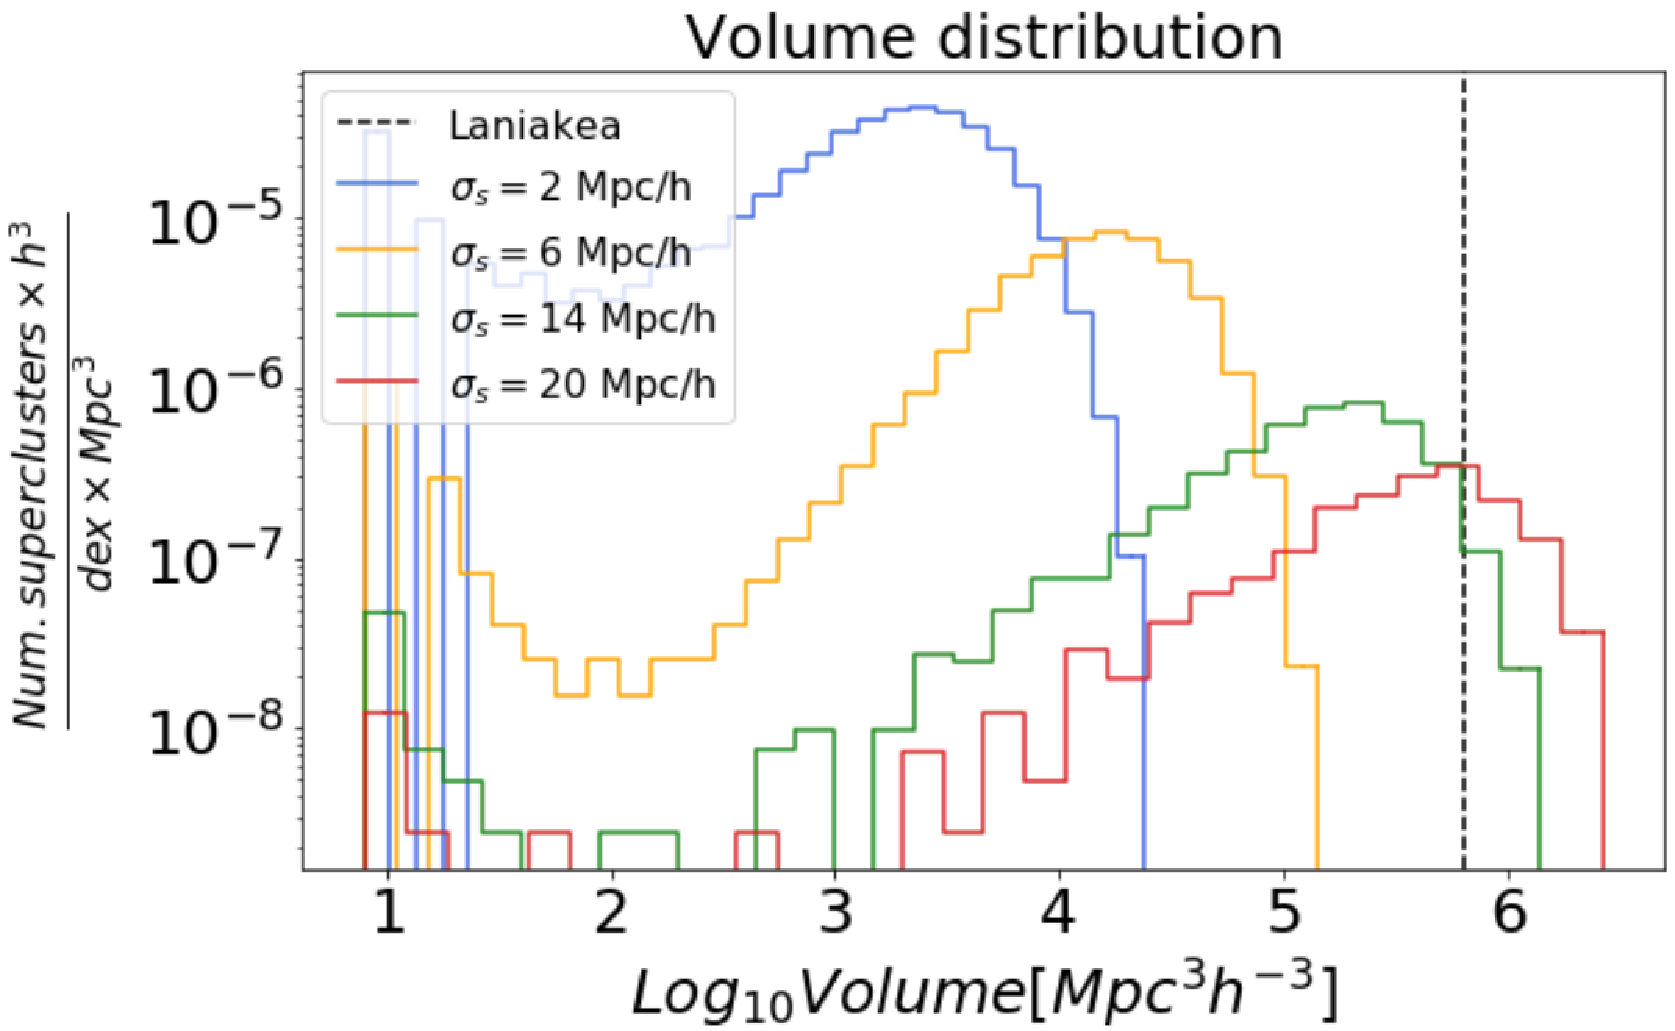
\includegraphics[width=345pt]{vol_different_sigmas.pdf}
    \caption{On this plot the volume of Laniakea is compared with the volumes of superclusters found using the watershed algorithm with different values of $\sigma_s$. A vertical line is showing the correspondent volume of Laniakea is also shown. The same AbacusCosmos\_720box\_planck simulation was smoothed using $\sigma_s$ = 2\,\Mpch, 6\,\Mpch, 14\,\Mpch and 20\,\Mpch and the volume distribution of the superclusters found is presented in this figure.} 
    \label{fig:HISTVMD2}
\end{figure*}




\subsection{Laniakea classification}

At this point, we have already seen that the volume distribution of the selected superclusters has a significant dependence on the choice of $\sigma_s$. Therefore, if we want to compare the classification made by the algorithm with reported volume measures of Laniakea, we must choose wisely the value of the Gaussian length. Thus, the value reported by \cite{2014Natur.513...71T} in his studies on CosmicFlows-2 data is used. From now on, the value of the Gaussian length is fixed and equals 10\Mpch. 

Now, in order to complete the analysis of Laniakea, it is important to establish a pattern by using different sets of simulations. We are interested in the impact that different cosmological parameters may have in the volume distribution of superclusters, as well as the behaviour of this distribution when different time evolution are considered.


\subsubsection{Planck 2015 parameters}

To begin with, a set of 5 simulations of the Abacus\_Cosmos\_720box\_planck catalog is considered. This set of simulations fulfills two main functions. First, it allows us to observe the effects of the time evolution on the resulting volume distribution. Second, as the simulations are executed using Planck 2015 cosmological parameters, we are able to establish a reference point with generally accepted cosmological parameters. In this way, figure \ref{fig:planck} shows the volume distributions of the superclusters found by Watershed algorithm using this data set. This chart also shows a vertical line where the reported volume of Laniakea is located. As expected from figure \ref{fig:1Pert}, Laniakea is larger than any other simulation found by the algorithm, and it does not change with different time evolution. For instance, the volume of our local supercluster is found on the right side and out of the distributions, which implies that there is no structure as big as Laniakea. Consequently, we conclude that Laniakea is an atypical supercluster if a normal cosmology is considered. \\



However, the atypical behaviour found using Planck 2015 parameters may change if extreme cosmologies are used in this process. The effect of the mass density of the universe ($\Omega_m$), as well as the value of the matter fluctuations in present time ($\sigma_8$) might cause volume distributions to be affected and, therefore, it can affect how typical or atypical Laniakea is. Thus it is important to consider different simulations that satisfy this extreme conditions.


\subsubsection{Extreme values of $\Omega_m$ and $\sigma_8$}

Now, a set of 4 simulations of the Abacus\_Cosmos\_720box catalog as well as an Abacus\_Cosmos\_720box\_planck reference simulation is studied. From Abacus\_Cosmos\_720box we extract the 4 simulations that correspond to the highest and lowest values of $\Omega_m$ and $\sigma_8$ found in this catalog. Thereby, the selected set contains the simulations with the highest value of $\sigma_8$ and $\Omega_m$ (0.999 and 0.367 respectively) and the lowest value of the same parameters (0.647 and 0.253 respectively). The resulting volume distributions for this data set are shown in figure \ref{fig:diferentes}. A vertical line representing the volume of Laniakea is shown too. We observe that even when extreme cosmologies are considered, the volume of Laniakea is located outside the distributions and, therefore, this supercluster conserves its atypical size and behaviour.



\begin{figure*}
    \centering
    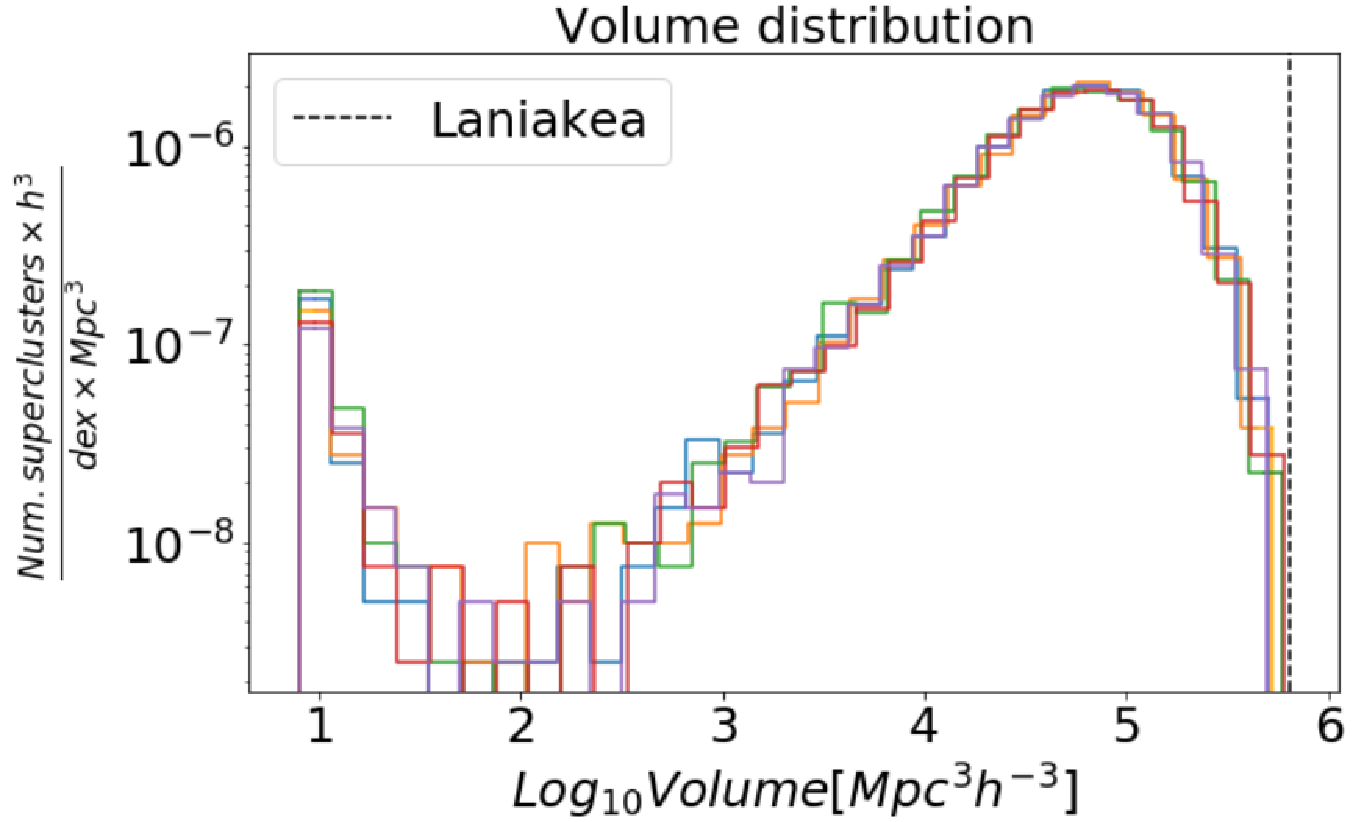
\includegraphics[width=345pt]{vol_planck.pdf}
    \caption{On this plot the volume of Laniakea is compared with the volumes of superclusters found using the watershed algorithm for 5 simulations using Planck parameters and $\sigma_s = 10$\,\Mpch. A vertical line is showing the correspondent volume of Laniakea is also shown. An atypical behaviour in the volume of Laniakea is observed as it is larger than most of the superclusters found by the algorithm. } 
    \label{fig:planck}
\end{figure*}


\begin{figure*}
    \centering
    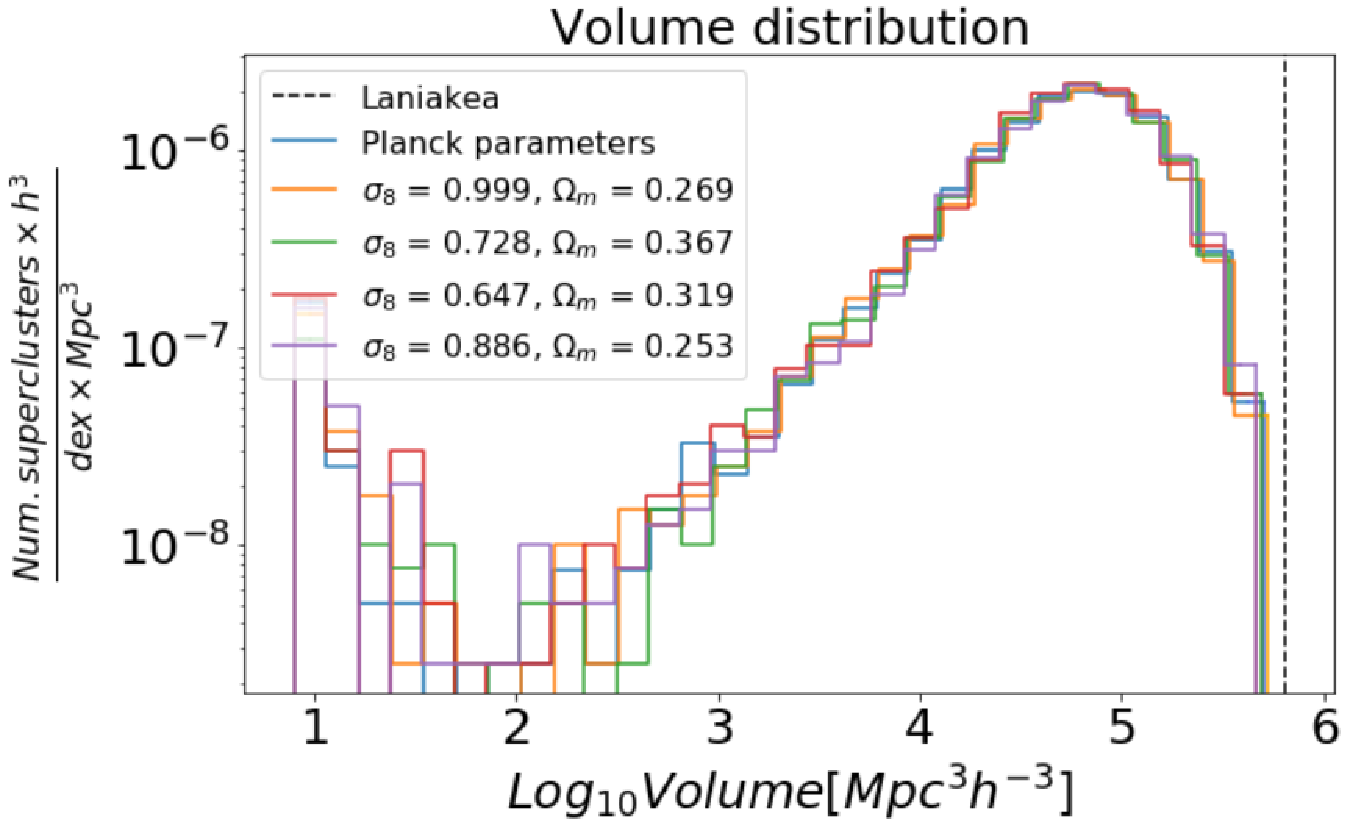
\includegraphics[width=345pt]{vol_different_simulations.pdf}
    \caption{On this plot the volume of Laniakea is compared with the volumes of superclusters found using the watershed algorithm for a set of 4 simulations from Abacus\_Cosmos\_720box catalog given by extreme values of $\sigma_8$ and $\Omega_m$. In addition, a reference simulation from Abacus\_Cosmos\_720box\_planck catalog is considered. A vertical line is showing the correspondent volume of Laniakea is also shown. The simulations used in this chart were smoothed using $\sigma_s = 10$\,\Mpch and the $\sigma_8$ and $\Omega_m$ values chosen are presented in the graph. An atypical behaviour in the volume of Laniakea is observed as it is larger than every supercluster found by the algorithm.} 
    \label{fig:diferentes}
\end{figure*}




\section{Conclusions}
\label{sec:conclusions}

A recent result in this branch was the definition of our local supercluster Laniakea made by \cite{2014Natur.513...71T}, who used the velocity flow of galaxies for this purpose. Already having the characteristics of Laniakea, both in form and in mass, the next question would be how common it is among the other superclusters.

We divide the space of the simulation with a grid size close to the canonical length of \texttt{10\,Mpc} used in observations to find Laniakea, which corresponds to a grid of [$120 \times 120 \times 120$]. Once the velocity field is obtained, it is smoothed with Gaussian kernels of different width $\sigma_{Vox}$. Then the VDC is computed for each gridpoint. In order to differentiate structures from the order of the observable superclusters i.e. structures of about 10\,\Mpch, we use $\sigma_{Vox} = 1$\,Vox. Using larger values of $\sigma_{Vox}$ does \texttt{NOT} yield erroneous information, but information with little usefulness about formation in a much larger scale.  

The implementation of the Watershed algorithm was a complete success. It managed to segregate regions based on the divergence field. Two parameters, $R_T$ and $Q_T$, are defined to control the algorithm and the segregation it makes. $R_T$ is of high relevance since it indirectly dictates the number of \emph{origins} that there are in the map and, therefore, the number of superclusters that will be in the space of the simulation. $Q_T$, on the other hand, does not affect the analysis carried out by the algorithm in a meaningful way since it rather indirectly defines the top of watershed sweeps that must be made before proceeding to classify the voxels by distance.

With the superclusters segregated and characterized we compare their propoerties against Laniakea. We find that our supercluster is  atypical according to its mass, volume and shape. On the other hand, the density of Laniakea seems to be frequent in the supercluster population since it is in a range close to the average. The populations with which Laniakea is compared within the simulation are small, either evaluating its mass, its volume or its shape. This makes it difficult to find a supercluster in the simulation that is similar to Laniakea within the ranges defined in Figures \ref{fig:HISTVMD1} and \ref{fig:INERTIA} at the same time. The probability of finding in the simulation a supercluster similar to Laniakea in those three aspects is a little lower than 0.07\,\%.

Regarding future work, we strongly suggest to experiment with the initial conditions of the problem and with the definition of the grid. A proposal is to define a grid with distances less than 10\,\Mpch, that is, with a higher value of $N_{side}$ and therefore with greater definition. You can also try different mass cuts for the Halos, different simulations of the same cosmology used in this work or even simulations in the context of different cosmologies.\\



\bibliographystyle{mnras}
\bibliography{references}



\end{document}
